\section{Intro}
There are a couple formalisms for mechanical problems:
\begin{itemize}
	\item Newtonian formalism. Focuses on forces.
	\item Lagrangian formalism. Focuses on Lagrangians. ''Actions``
	\item Hamiltonian or canonical formalism. Focuses on Hamiltonians.
\end{itemize}

Topics:
\begin{itemize}
	\item Lagrangian formalism
	\item Small oscillation
	\item Hamiltonian formalism
	\item Central forces. Kepler problems.
	\item Rigid body movement
\end{itemize}

\section{Lagrangian formalism}
\begin{itemize}
	\item Intro
	\item Lagrangian $ L $ and derivation of Euler-Lagrange equations. 
	\item Principle of least action - define action based on Lagrangian. On physical trajectory action will be minimal. Physical trajectory is solution of Euler-Lagrange equations. 
\end{itemize}

\subsection{Definition of mechanical problem}
Given $N$ bodies and forces acting on them. Each body can be described with its position $\mathbf{r}_i$. Solution of the problem is $\mathbf{r}_i(t)$, i.e. position as function of time.

\paragraph{Number of degrees of freedom} is number of parameters needed to describe the system. We need 2 numbers to describe each degree of freedom.
\paragraph{Configuration space} is space of all possible states of system. For $N$ degrees of freedom we have $N$-dimensional configuration space. Solution of mechanical problem is a path in configuration space.
\paragraph{Example}
Two springs. Configuration space is 2D. If we have only one spring moving, that'd be a line parallel to one of the axis. For more general case, if springs are identical, we get ellipse.

\begin{center}
	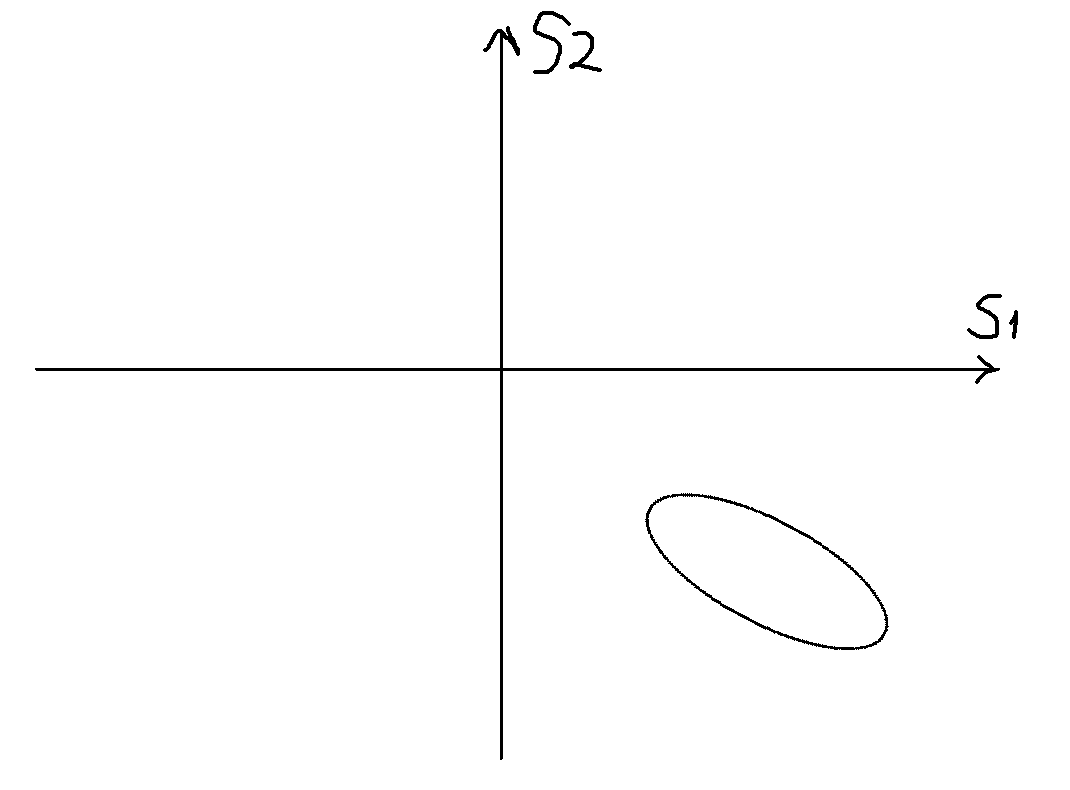
\includegraphics[width=0.5\linewidth]{./lect1/1.png}
\end{center}

\subsection{Lagrangian}
Let's describe the system with Lagrangian, which is function of coordinates, velocities and time.

Starting with one-particle system. Kinetic energy: $T(\dot{\vec{r}})=\frac{1}{2}m\dot{\vec{r}}^2$. Potential energy: $V(\vec{r}, t)$. Define
$$L(\vec{r}, \dot{\vec{r}}, t) = T(\dot{\vec{r}}) - V(\vec{r},t)$$
Derive Euler-Lagrange equations from Lagrangian:
$$\frac{d}{dt}\left( \frac{\partial}{\partial \dot{r}_\alpha} L(\vec{r}, \dot{\vec{r}}, t) \right) = \frac{\partial}{\partial r_\alpha} L(\vec{r}, \dot{\vec{r}}, t) $$
Since $L(\vec{r}, \dot{\vec{r}}, t) = T(\dot{\vec{r}}) - V(\vec{r},t)$:

$$\frac{\partial L}{\partial \dot{r}_\alpha} = \frac{\partial T}{\partial \dot{r}_\alpha} = \frac{\partial}{\partial \dot{r}_\alpha} \left[ \sum_{\beta} \frac{1}{2}m\dot{r}^2_p \right] = m\dot{r}\beta$$
$$\frac{d}{dt} \left( \frac{\partial L}{\partial \dot{r}_\alpha} \right) = m\ddot{r}_\alpha $$
$$\frac{\partial L}{\partial dr_\alpha} = -\vec{\nabla} V$$
We got Newton law:
$$m\ddot{\vec{r}} = -\vec{\nabla} V$$
\paragraph{Note} In different coordinates, $T$ might depend not only on velocities. For example, kinetic energy of a particle in spherical coordinates is $T = \frac{m}{2}\left[\dot{r}^2 + r^2\dot{\theta}^2 + r^2 \sin^2 \theta \cdot \dot{\varphi}^2 \right]$.

\paragraph{Multi particle system} For N particles:
$$L(\vec{r}_1,\dots, \vec{r}_N, \dot{\vec{r}}_1,\dots, \dot{\vec{r}}_N,t) = \sum_i \frac{1}{2} m_i \dot{\vec{r}}_i - V(\vec{r}_1,\dots, \vec{r}_N, t)$$

In this course we talk only on conserving forces. Meanwhile the potential is independent on velocity.

\paragraph{Example} Spring. $F_{spring} = kx$.
$$L(x, \dot{x}) = \frac{1}{2}m\dot{x}^2 - \frac{1}{2}kx^2$$
$$\frac{\partial L}{\partial x} = -kx$$

$$\frac{d}{dt}\left(\frac{\partial L}{\partial \dot{x}}\right) = \frac{d}{dt} m\dot{x} = m\ddot{x}$$

\subsection{Principle of least action}
Given the system described with Lagrangian
$$L(\vec{r}(t), \dot{\vec{r}}(t),t)= T_V$$
Lets take a look at path in configuration space:  \begin{wrapfigure}{R}{0.3\textwidth}
	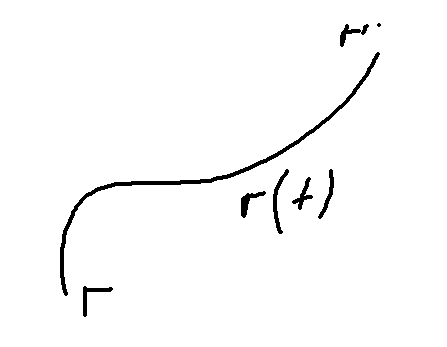
\includegraphics[width=\linewidth]{./lect1/2.png}
\end{wrapfigure}

Define action $S$ as
$$S\left[r(t)\right] = \int_{\tau_1}^{\tau_2} L(\vec{r}(t), \dot{\vec{r}}(t),t) dt$$
$S$ is functional, i.e. function whose parameter is function.
\paragraph{Note} Path $r(t)$ contains not only geometrical path but also the pace, i.e. if $q(\tau_1) = Q$ and $q(\tau_2)=Q^\prime$, there are different paths from $Q$ to $Q^\prime$ with different paces.
\paragraph{Principle of least action} Physical system described with Lagrangian $L$ will move in configuration space on path with minimal action $S$.

We'll show that Euler-Lagrange equations are necessary for existence of such path. We'll use principle of variation which is a way to find minimum of functional. Euler-Lagrange is acquired from principle of variation.